%% Aspect ratio 16:10, delete for 4:3
\documentclass[compress,english,aspectratio=1610]{beamer}

\usepackage[english]{babel}
\usepackage[T1]{fontenc}
\usepackage[utf8]{inputenc}
\usepackage{graphicx}
\usepackage{tcolorbox}
\usepackage{ulem}
\usepackage{listings}
%\usepackage{pgfplots}
%\usepackage{relsize}

\setcounter{secnumdepth}{3}
\setcounter{tocdepth}{3}

%\pgfplotsset{compat=1.5, width=13cm, height=7cm}
\setbeamertemplate{caption}{\raggedright\insertcaption\par} % no "Figure X in captions"
\setbeamercovered{transparent}

    \expandafter\def\expandafter\insertshorttitle\expandafter{%
      \insertshorttitle\hfill%
      \insertframenumber\,/\,\inserttotalframenumber}

%% Evenly spread items
\let\olditem\item
\renewcommand{\item}{\setlength{\itemsep}{\fill}\olditem}

%% MPG green (Pantone 328)
\definecolor{mpg-green}{cmyk}{1,0,0.57,0.3}
\definecolor{mpg-gray}{cmyk}{0,0,0.06,0.23}

%% Symbols for footnotes
\renewcommand*{\thefootnote}{\fnsymbol{footnote}}

\newcommand{\Cpp}{C\texttt{++}}


\hypersetup{
  colorlinks,
  allcolors=.,
  urlcolor=blue,
}

\mode<presentation>
 {
  \usetheme{Ilmenau}
  %% Beamer color theme
  \usecolortheme[cmyk={1,0,0.57,0.3}]{structure}
  %% use MPG green also for alerted text
  \setbeamercolor{alerted text}{fg=mpg-green}
  \setbeamercolor{itemize item}{fg=mpg-gray}
  \beamertemplatenavigationsymbolsempty{}
  %\setbeamertemplate{footline}[frame number]
}

    \setbeamerfont{section title}{parent=title}
    \setbeamercolor{section title}{parent=titlelike}
    \defbeamertemplate{section page}{mine}[1][] {%
      \centering
        \begin{beamercolorbox}[sep=8pt,center,#1]{section title}
          \usebeamerfont{section title}\insertsection\par
        \end{beamercolorbox}
    }
%    \newcommand*{\mysectionpage}{\usebeamertemplate*{section page}}

\setbeamertemplate{section page}[mine]

\AtBeginSection[]{\subsection{}\frame{\sectionpage}}

\AtBeginSection[]
{
  \begin{frame}<beamer>
    \frametitle{Outline}
    \tableofcontents[currentsection]
  \end{frame}
}

%\usepackage{tikz}

%\newcommand{\bluecheck}{}%
%\DeclareRobustCommand{\greencheck}{%
%  \tikz\fill[scale=0.4, color=mpg-green]
%  (0,.35) -- (.25,0) -- (1,.7) -- (.25,.15) -- cycle;%
%}

\usepackage{amssymb}% http://ctan.org/pkg/amssymb
\usepackage{pifont}% http://ctan.org/pkg/pifont
\newcommand{\cmark}{{\color{mpg-green}\ding{51}}}%
\newcommand{\xmark}{{\color{red}\ding{55}}}%

\setbeamercovered{invisible}

\newcommand\redout{\bgroup\markoverwith{}
{\textcolor{red}{\rule[.5ex]{4pt}{2pt}}}\ULon}

\usepackage[edges]{forest}
\definecolor{folderbg}{RGB}{124,166,198}
\definecolor{folderborder}{RGB}{110,144,169}
\newlength\Size{}
\setlength\Size{4pt}
\tikzset{%
  folder/.pic={%
    \filldraw [draw=folderborder, top color=folderbg!50, bottom color=folderbg] (-1.05*\Size,0.2\Size+5pt) rectangle ++(.75*\Size,-0.2\Size-5pt);
    \filldraw [draw=folderborder, top color=folderbg!50, bottom color=folderbg] (-1.15*\Size,-\Size) rectangle (1.15*\Size,\Size);
  },
  file/.pic={%
    \filldraw [draw=folderborder, top color=folderbg!5, bottom color=folderbg!10] (-\Size,.4*\Size+5pt) coordinate (a) |- (\Size,-1.2*\Size) coordinate (b) -- ++(0,1.6*\Size) coordinate (c) -- ++(-5pt,5pt) coordinate (d) -- cycle (d) |- (c) ;
  },
}
\forestset{%
  declare autowrapped toks={pic me}{},
  pic dir tree/.style={%
    for tree={%
      folder,
      font=\ttfamily,
      grow'=0,
    l sep=0.5cm,
    s sep=0.1cm,
    minimum height=0.1cm,
    minimum width=1cm,
    },
    before typesetting nodes={%
      for tree={%
        edge label+/.option={pic me},
      },
    },
  },
  pic me set/.code n args=2{%
    \forestset{%
      #1/.style={%
        inner xsep=2\Size,
        pic me={pic {#2}},
      }
    }
  },
  pic me set={directory}{folder},
  pic me set={file}{file},
}

\title{\textbf{Good practices for Python development} \\ \textit{What you should know before doing anything}}
\author{ZWE Software Workshop}
\institute{Max-Planck-Institut f\"ur Intelligente Systeme \vspace{3.5cm}}
\date{\small{MPRIS Workshop, 28 October, 2021}}

\begin{document}
%% Title frame
\begin{frame}[plain,label=thetitle]
 \titlepage
\end{frame}

\logo{
\includegraphics[height=1cm]{figures/minerva}}


%% Table of Contents
\begin{frame}{Outline}
	\tableofcontents
\end{frame}


% Project structure
\section{Project structure and content}

\begin{frame}
\frametitle{Where do I start?}
  You start a new project. What do you need to do and what should be there at the bare minimum.
\end{frame}

\begin{frame}{Minimal structure}
  \begin{forest}
  pic dir tree,
  where level=0{}{% folder icons by default; override using file for file icons
    directory,
  },
  [project
  	[doc
  	]
    [package
      [\_\_init\_\_.py, file
      ]
      [version.py, file
      ]
      [..., file
      ]
    ]
    [tests
    ]
    [LICENSE.md, file
    ]
    [README.md, file
    ]
    [requirements.txt, file
    ]
    [setup.py, file
    ]
  ]
\end{forest}
\end{frame}

\begin{frame}[fragile]
  \frametitle{README.md}

  This is the first thing people read. \texttt{github}, \texttt{gitlab}, etc.~display this on the project page. It should contain:
  \begin{itemize}
  \item project name
  \item project description
  \item requirements (but not python dependencies)
  \item installation instructions
  \item maybe usage examples
  \end{itemize}
\end{frame}

\begin{frame}[fragile]
  \frametitle{LICENCE}
  This license explains what people can do with your code. Pick the one you see fit (MIT, BSD, etc) and just copy it in your repo.
\end{frame}

\begin{frame}[fragile]
  \frametitle{.gitignore}
  (not pictured in the previous slide)

  This file lists all the file \textit{patterns} \texttt{git} should ignore. It's a good idea to put in there all the \texttt{\_\_pycache\_\_} and \texttt{*.pyc} and \texttt{*.so} and \texttt{.idea} and so on.

  If you don't know what to put in there, \texttt{github} offers you a truly all-encompasing file when creating a repo.
\end{frame}

\begin{frame}[fragile]
\frametitle{Github offers those three for you}
  \begin{figure}
    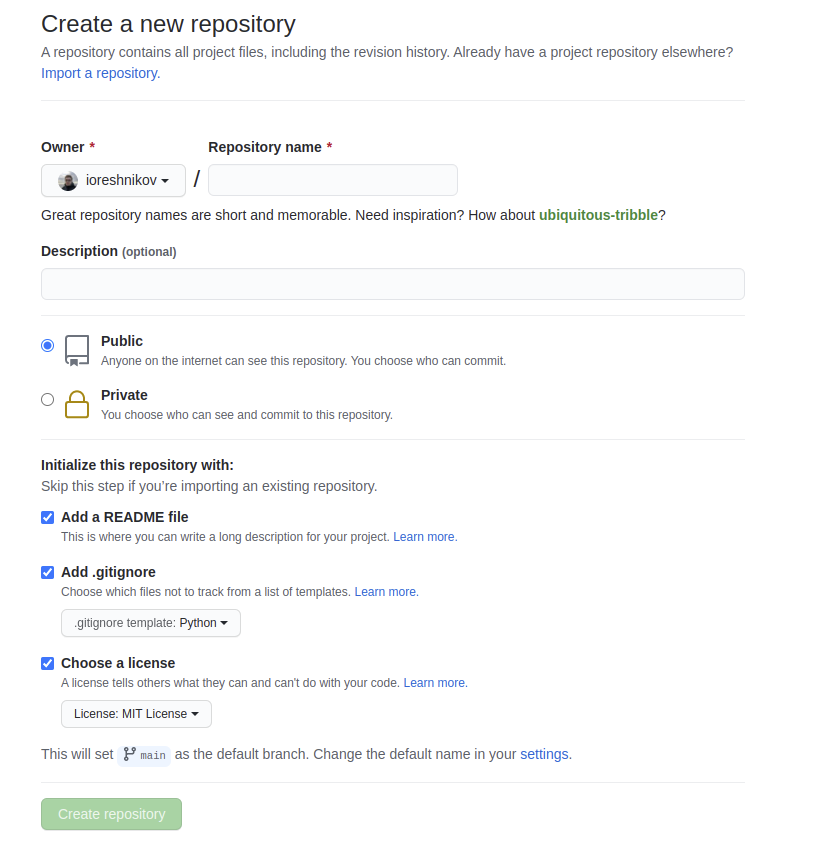
\includegraphics[width=0.5\textwidth]{figures/new_repo_form.png}
  \end{figure}
\end{frame}


\begin{frame}[fragile]
  \frametitle{Requirements file}
  The {\tt requirements.txt} file contains the list of the dependencies of your project that can be installed via {\tt pip}:
  \begin{tcolorbox}[colback=mpg-gray,colframe=mpg-green,title=Contents of requirements file]
	{\tt numpy}\\
	{\tt scipy}\\
	{\tt matplotlib==3.1.1}\\
	{\tt mock>=3.0}\\
	{\tt pywin32; sys\_platform == 'win32'}
  \end{tcolorbox}

  Usage:
  \begin{tcolorbox}[colback=mpg-gray,colframe=mpg-green,title=Commands]
	{\tt \$ pip install -r requirements.txt}
  \end{tcolorbox}
\end{frame}


\begin{frame}[fragile]
  \frametitle{setup.py}
  The {\tt setup.py} file describe your project and allows you to build/distribute it:
  \begin{tcolorbox}[colback=mpg-gray,colframe=mpg-green,title=Contents of setup file]
	{\tt from setuptools import setup}\\
	{\tt setup(name=package\_name, version=1.0, \verb|\|}\\
	{\tt install\_requires=['numpy'], zip\_safe=False)}
  \end{tcolorbox}

  Usage:
  \begin{tcolorbox}[colback=mpg-gray,colframe=mpg-green,title=Commands]
	{\tt \$ pip install . \# install as a package}\\
	{\tt \$ pip install -e . \# for development}\\
	{\tt \$ python setup.py sdist \# build a source distribution}\\
	{\tt \$ python setup.py build\_ext bdist\_wheel \# build a wheel}
  \end{tcolorbox}
\end{frame}

\begin{frame}[fragile]
  \frametitle{Example project}
  We have set up a minimal (more or less) real-world example you can use as a reference

  \begin{center}
    \href{https://github.com/MPI-IS/py-project-example}{github.com/MPI-IS/py-project-example}
  \end{center}
\end{frame}

\begin{frame}[fragile]
\frametitle{What about the data?}
  \begin{itemize}
  \item If it's small and you have no licensing problems you might as well put it in the repository, for example in a separate directory named \texttt{data/}.
  \item If you don't want to commit it, it's still a good idea to put it in the \texttt{data/} directory. How not to commit by accident: create an empty file \texttt{data/.keep}, commit \textit{this file only}, put the entire content of \texttt{data/*} in \texttt{.gitignore} and then copy the data in that directory.
  \end{itemize}
\end{frame}

\begin{frame}
\frametitle{What about the scripts?}
  Where to put the scripts, for example to train and evaluate the model?
  \begin{itemize}
  \item create a \texttt{scripts/} directory and put your scripts there
  \item add them to a \texttt{scripts=[]} section in \texttt{setup.py}
  \item after \texttt{pip install -e .} they should be visible in the environment \textit{globally}, i.e.~independent from the working directory. The imports will also work.
  \end{itemize}
\end{frame}

\begin{frame}
  \centering
  Questions so far?
\end{frame}


\section{Virtual environments}

\begin{frame}{The problem}
  \begin{itemize}
    \item By default, you are using a single Python interpreter for all your projects.
	\item If you install your packages with the corresponding {\tt pip},
		there is a high chance you will \textbf{create conflicts} between your projects
  \end{itemize}
  Solutions:
  \only<1>{Edit your {\tt PYTHONPATH}, {\tt .bashrc}, {\tt .profile}, brew python...}
  \only<2>{\redout{Edit your {\tt PYTHONPATH}, {\tt .bashrc}, {\tt .profile}, brew python...}}

  \begin{figure}
    \includegraphics<2->[width=0.35\textwidth]{figures/python_environment.png}
  \end{figure}
\end{frame}

\begin{frame}[fragile]
  \frametitle{Virtual environments}
  The \textbf{correct solution} is to use virtual environments.

  A \textbf{virtual environment} is a \textbf{local} Python environment that is \textbf{isolated}
  from other virtual environments and (by default) from the system Python.
  Advantages:
  \begin{itemize}
    \item no sudo rights needed
  	\item it has its own {\tt python}, {\tt pip}...
  	\item whatever you install stays in the virtual environment
  	\item if something goes wrong, delete the folder and create a new one
  \end{itemize}

  Usage:
  \begin{tcolorbox}[colback=mpg-gray,colframe=mpg-green,title=Commands]
	{\tt \textasciitilde/Code/my-project\$ python3 -m venv \texttt{-{}-}copies my\_venv}\\
	{\tt \textasciitilde/Code/my-project\$ . my\_venv\verb|\|bin\verb|\|activate}\\
	{\tt (my\_venv) \textasciitilde/Code/my-project \$ which python}\\
	{\tt (my\_venv) \textasciitilde/Code/my-project \$ deactivate}
  \end{tcolorbox}
\end{frame}

\begin{frame}[fragile]
  \frametitle{A convinience: pipenv}
  If this one seems clunky, use \href{https://github.com/pypa/pipenv}{\texttt{Pipenv}}! It allows you to create and activate the environment based on your working directory.
  \begin{tcolorbox}[colback=mpg-gray,colframe=mpg-green,title=Commands]
	{\tt \textasciitilde/Code/my-project\$ pipenv install}\\
	{\tt \textasciitilde/Code/my-project\$ pipenv shell}\\
	{\tt (my\_venv) \textasciitilde/Code/my-project \$ which python}\\
	{\tt (my\_venv) \textasciitilde/Code/my-project \$ deactivate}
  \end{tcolorbox}
\end{frame}

\begin{frame}
  \frametitle{If you must: conda}
  \href{https://docs.conda.io/en/latest/}{\texttt{Conda}} is a distribution and a package manager and an environment manager wrapped in one. It's really popular among data scientists and machine learning researchers and egineers.
  \vskip 1cm
  We personally do not use it. Sometimes with \texttt{conda} things break in a strange way. But if you have to (need a very tricky set of exactly versioned dependencies, difficult installation with many third-parties, you are on Windows, etc.), then please do.
\end{frame}

\begin{frame}
  \centering
  Questions so far?
\end{frame}


\section{Code style}

\begin{frame}
  \frametitle{Code can look differently}
  The same problem can be solved in many different ways. The algorithms might be different. But even the way the same algorithm \textit{looks} might be also different.
\end{frame}

\begin{frame}
  \frametitle{Examples}
  \begin{itemize}
  \item How do we name variables? And how do we spell the names? \texttt{like\_so} or \texttt{MaybeLikeSo}?
  \item How do we name functions? Is it \texttt{is\_even(number)} or \texttt{even(number)}? And again, why not \texttt{IsEven(number)}?
  \item Where do we put braces? How do we break long lines? What's a long line anyway? Tabs or whitespaces?
  \item Sometimes it's technical, e.g. do we throw exceptions?
  \end{itemize}
\end{frame}

\begin{frame}
  \frametitle{Ideally we want the code to look the same}
  If there are several people working on the project it is good idea to make the code at least look the same way.
  \begin{itemize}
  	\item consistency --- there should be few surprises when switching from one part of the project to another, because
  	\item readability --- once you have a consistent style you can get used to it and the code will be easier to read and as a result
  	\item comprehension --- you will understand more
  \end{itemize}
\end{frame}

\begin{frame}
  \frametitle{Code style}
  The way engineers do it is by introducing a \textit{code style}. Agree on the common way to write the code and try to keep it this way. The scope can be different
  \begin{itemize}
  \item almost always there is a code style specific to the project. See \href{https://www.kernel.org/doc/html/v4.10/process/coding-style.html}{Linux Kernel Style Guide} (for C).
  \item sometimes there is a company-wide style. See \href{https://google.github.io/styleguide/cppguide.html}{Google Style Guide} (for C++).
  \item sometimes there is an official style guide for a specific language. This usually also means that one can write tools that help to keep the style.
  \item the most radical: there is a \textit{very opinionated} official style guide and there are powerful out-of-the-box tools doing the job for you. See \href{https://go.dev/blog/gofmt}{go fmt} and \href{https://github.com/rust-lang/rustfmt}{rustfmt}.
  \end{itemize}
\end{frame}

\begin{frame}
  \frametitle{PEP8}
  Python has an official style guide known as \href{https://www.python.org/dev/peps/pep-0008}{PEP8}.
\end{frame}

\begin{frame}
  \frametitle{(interlude) What's a PEP}
  \texttt{PEP} is a python enhancement proposal. A few examples:
  \begin{itemize}
  	\item \href{https://www.python.org/dev/peps}{PEP0}: Index of PEPs
  	\item \href{https://www.python.org/dev/peps/pep-0020}{PEP20}: The Zen of Python
  	\item \href{https://www.python.org/dev/peps/pep-0257}{PEP257}: Docstring Conventions
    \item \href{https://www.python.org/dev/peps/pep-0465}{PEP465}: A dedicated infix operator for matrix multiplication
  \end{itemize}
\end{frame}

\begin{frame}
  \frametitle{PEP8}
  Python has an official style guide known as \href{https://www.python.org/dev/peps/pep-0008}{PEP8}. It is 10 to 20 pages long and it illustrates how to write and how not to write python code.
\end{frame}

\begin{frame}{Tools to help you}
  There are some tools to help you with code style:
  \begin{itemize}
  	\item standalone style checkers such as \href{http://flake8.pycqa.org/en/latest/}{flake8}
  	\item formatters such \href{https://github.com/psf/black}{black} as \href{https://pypi.org/project/autopep8/0.8/}{autopep8}
  	\item if you want to be strict/annoying, then such checker/formatters can be used as a \href{https://git-scm.com/docs/githooks}{githook}
  	\item most IDEs have plugins that use those tools automatically. PyCharm does this out-of-the-box. VSCode/Atom do that when you install a python extension. There are ways to integrate this into VIM/Emacs.
  \end{itemize}
\end{frame}

\begin{frame}
  This is only about the style.
  \vskip 1cm
  There are code analyzers that are a bit more advanced, e.g. \href{https://pylint.org/}{pylint} or \href{https://pypi.org/project/radon/}{radon}.
\end{frame}

\begin{frame}{There is no silver bullet}
  This is the bare minimum, but it does not guarantee your code any good.
  \begin{itemize}
  \item tools do not help with the overall sanity of your naming scheme.
  \item tools do not help you to structure your code into functions/classes/modules either.
  \item tools cannot guarantee that the code is straightforward enough.
  \item in the end you can write a good code but it doesn't look \textit{idiomatic}!
  \end{itemize}
\end{frame}

\begin{frame}
  \centering
  It is difficult to define what a good code is.
\end{frame}

\begin{frame}{It is a skill}
  Writing good code is a skill. It can be learned and it can be taught. Mostly by example.
  \begin{itemize}
  \item there are books. Python-specific --- a (free online, a bit chaotic) Chapter on \href{https://docs.python-guide.org/\#writing-great-python-code}{writing great python code} in The Hitchhiker's Guide to Python. In general --- Clean Code: A Handbook of Agile Software Craftsmanship.
  \item read good code
  \item do \textit{code reviews}, i.e.~write bad code, show it to other people and ask for their opinion
  \end{itemize}
\end{frame}

\begin{frame}
  We do code reviews as a service. If you have a project you want to publish and you are not sure whether it is good or how to improve it then we are happy to help. Caveat: we might be slow, so write us in advance.
\end{frame}

\begin{frame}
  \centering
  Questions so far?
\end{frame}

\end{document}

%%% Local Variables:
%%% mode: latex
%%% TeX-master: t
%%% End:
